\documentclass[math0540-lecture-notes.tex]{subfiles}
\begin{document}

\chapter{Inner Product Spaces}

With vector spaces, we generalized the linear structure (of addition and scalar multiplication) in
$\R^2$ and $\R^3$; however, we ignored other important features, such as length and angle. We now
explore these ideas through \textbf{inner products}.

\section{Inner Products and Norms}
\subsection{Inner Products}

To motivate inner products, let's recall vectors in $\R^2$. The length of a vector $\vec{v}\in \R^2$
is called the \textbf{norm} of $\vec{v}$, denoted $\|\vec{v}\|$; and we calculate the norm of a
vector $\vec{v}=(x_1,x_2)$ as follows: \[
  \|\vec{v}\|=\sqrt{x_1^2+x_2^2}
.\] Similarly, if $\vec{v}=(x_1,x_2,x_3)\in \R^3$, then \[
  \|\vec{v}\|=\sqrt{x_1^2+x_2^2+x_3^2}
.\] Even though we can't visualize vectors in higher dimensions, the generalization to $\R^n$ is
clear: for a vector $\vec{v}=(x_1,x_2,\ldots,x_n)\in \R^n$, the norm of $\vec{v}$ is \[
  \|\vec{v}\|=\sqrt{x_1^2+x_2^2+\ldots+x_n^2}
.\] However, clearly the norm is not linear on $\R^n$. To achieve this linearity, we introduce the
\textbf{dot product}.

\begin{definition}[Dot Product]{}
  For $x,y\in \R^n$, the \textbf{dot product} of $x$ and $y$, denoted $x\cdot y$, is \[
    x\cdot y=x_1y_1+\ldots+x_ny_n
  ,\] where $x=(x_1,\ldots,x_n)$ and $y=(y_1,\ldots,y_n)$.
\end{definition}

Importantly, the dot product of two vectors of $\R^n$ is a number, \textbf{not} a vector. Clearly,
\[
  x\cdot x=\|x\|^2
\] for all $x\in \R^n$. The dot product has the following properties:
\begin{itemize}
  \item $x\cdot x\ge 0$ for all $x\in \R^n$.
  \item $x\cdot x=0$ if and only if $x=0$.
  \item For $y\in \R^n$ fixed, the map from $\R^n$ to $\R$ that sends $x\in \R^n$ to $x\cdot y$ is
    linear.
  \item $x\cdot y=y\cdot x$ for all $x,y\in \R^n$.
\end{itemize}

Now, how might we generalize the dot product from $\R^n$ to a general vector space? An intuitive
notion may simply be to abstract the properties listed above. However, while this works for real
vector spaces, we want a definition that works for complex vector spaces as well. We introduce the
notion of \textbf{inner products}, but first, a review of complex numbers.

\begin{definition}[Complex Conjugates]{}
  Suppose $z=a+bi\in \C$. The \textbf{complex conjugate of $z$}, denote $\overline{z}$, is defined
  as \[
    \overline{z}=a-bi\in \C
  .\] Thus $z=\overline{z}$ if and only if $z\in \R$, i.e. $z=a+0i$ for some $a\in \R$.
\end{definition}

Note that complex conjugates respect addition and multiplication, in that \[
  \overline{z+w}=\overline{z}+\overline{w} ~\text{and}~ \overline{zw}=\overline{z}\overline{w}
\] for $z,w\in \C$. In other words, complex conjugation is an isomorphism between complex numbers.

\begin{definition}[Norm of Complex Number]{}
  The \textbf{absolute value}, or \textbf{norm}, of $z=a+bi$ is \[
    \left| z \right| =\sqrt{a^2+b^2}=\sqrt{(a+bi)(a-bi)}=\sqrt{z\overline{z}}
  .\] 
\end{definition}
Absolute values respect multiplication, i.e. $\left| zw \right| =\left| z \right| \left| w \right|$,
but \textbf{not} addition! See the section on triangle inequalities for absolute values and
addition.




\begin{definition}[Inner Product]{}
  An \textbf{inner product} on $V$ is a function that takes each ordered pair $(u,v)$ of elements of
  $V$ to a number $\left<u,v \right>\in \F$ and has the following properties:
  \begin{itemize}
    \item \textbf{Positive Definiteness}: $\left<v,v \right> \ge 0$ for all $v\in V$, and $\left<v,v
      \right>=0$ if and only if $v=0$.
    \item \textbf{Conjugate Symmetry}: $\left<u,v \right> = \overline{\left<v,u \right>}$ for all
      $u,v\in V$ (note that every real number equals its complex conjugate).
    \item \textbf{Linearity}: $\left<u+v,w \right> = \left<u,w \right>+\left<v,w \right>$ for all
      $uv,w\in V$, and $\left<\lambda u,v \right>=\lambda\left<u,v \right>$ for $\lambda\in \F$.
  \end{itemize}
\end{definition}

\begin{example}
  Here are some examples of inner products:
  \begin{itemize}
    \item The \textbf{Euclidean inner product} on $\F^n$, defined by \[
        \left<(w_1,\ldots,w_n),(z_1,\ldots,z_n) \right>=w_1\overline{z_1}+\ldots+w_n\overline{z_n}
      .\] If $\F$ is real, this is simply the dot product. If $c_1,\ldots,c_n$ are positive numbers,
      then the Euclidean inner product can be extended to \[
          \left<(w_1,\ldots,w_n),(z_1,\ldots,z_n)
          \right>=c_1w_1\overline{z_1}+\ldots+c_nw_n\overline{z_n}
      .\] 
  \item An inner product can be defined on the vector space of continuous real-valued functions on
    the interval $[-1,1]$ by \[
      \left<f,g \right>=\int_{-1}^1 f(x)g(x)dx
    .\] With polynomials, a similar inner product may be defined \[
    \left<p,q \right> = \int_0^\infty p(x)q(x)e^{-x}dx
    .\] 
  \end{itemize}
\end{example}

Inner products exist over vector spaces; we give these vector spaces a name.
\begin{definition}[Inner Product Spaces]{}
  An \textbf{inner product space} is a vector space $V$ along with an inner product on $V$.
\end{definition}

The most prominent example of an inner product space is $\F^{n}$ with the Euclidean inner product,
as defined above. When $\F^{n}$ is referred to as an inner product space, assume the inner product
is the Euclidean inner product unless explicitly told otherwise.

For notational convenience, too, we now denote $V$ an inner product space over $\F$.

\begin{proposition}[Properties of Inner Products]{}
  \begin{itemize}
    \item For each fixed $u\in V$, the function that takes $v$ to $\left<v,u \right>$ is a linear
      map from $V$ to $\F$.
    \item $\left<0,u \right>=0$ for every $u\in V$.
    \item $\left<u,0 \right> = 0$ for every $u\in V$.
    \item $\left<u,v+w \right> = \left<u,v \right>+\left<u,w \right>$ for all $u,v,w\in V$. For
      $\lambda\in \F$, $\left<u,\lambda v \right>=\overline{\lambda}\left<u,v \right>$. In other
      words, an inner product is \textbf{conjugate-linear} in the second term.
  \end{itemize}
\end{proposition}
\begin{proof}[Proof]
  (1) follows from the conditions of linearity in the first term for inner products. (2) follows
  from (1), since every linear map takes $0$ to $0$. (3) follows from (1) and the conjugate symmetry
  property of linear maps.

  For (4), suppose $u,v,w\in V$. Then
  \begin{align*}
    \left<u,v+w \right> &= \overline{\left<v+w,u \right>} \\
                        &= \overline{\left<v,u \right>+\left<w,u \right>} \\
                        &= \overline{\left<v,u \right>}+\overline{\left<w,u \right>} \\
                        &=\left<u,v \right>+\left<u,w \right>
                      .\end{align*} For (5), suppose $u,v\in V,\ \lambda\in \F$. Then
  \begin{align*}
    \left<u,\lambda v \right> &= \overline{\left<\lambda v,u \right>} \\ 
    &= \overline{\lambda\left<v,u \right>} \\
    &= \overline{\lambda} \overline{\left<v,u \right>}\\
    &=\overline{\lambda}\left<u,v \right>
  .\end{align*}
\end{proof}

\subsection{Norms}

Our motivation for defining inner products came initially from the norms of vectors in $\R^2$ and
$\R^3$, which represented the ``length'' of a vector. Now, we see that each inner product determines
a norm.
\begin{definition}[Norm]{}
  For $v\in V$, the \textbf{norm} of $v$, denoted $\|v\|$, is defined by \[
    \|v\|=\sqrt{\left<v,v \right>}
  .\] 
\end{definition}

Example norms include the standard norm on $\F^{n}$, where \[
  \|(z_1,\ldots,z_n)\|=\sqrt{\left| z_1 \right|^2+\ldots+\left| z_n \right| ^2 }
.\] In the vector space of continuous real-valued functions on $[-1,1]$ (with inner product defined
above), we have \[
  \|f\|=\int_{-1}^{1}(f(x))^2dx 
.\]

Now, let's look at some basic properties of norms.
\begin{proposition}[Properties of Norms]{}
  Suppose $v\in V$.
  \begin{enumerate}
    \item $\|v\|=0$ if and only if $v=0$.
    \item $\|\lambda v\|=\left| \lambda \right| \|v\|$ for all $\lambda\in \F$.
  \end{enumerate}
\end{proposition}
\begin{proof}[Proof]
  (1) follows directly from inner products, since $\left<v,v \right> = 0$ if and only if $v=0$.
  Suppose $\lambda\in \F$. Then
  \begin{align*}
    \|\lambda v\|^2&=\left<\lambda v,\lambda v \right>\\
                   &= \lambda\left<v,\lambda v \right>\\
                   &=\lambda\overline{\lambda}\left<v,v \right>\\
                   &=\left| \lambda \right| ^2\|v\|^2
  .\end{align*} Taking square roots now gives the desired equality.
\end{proof}

The above proof also illustrates that in general, working with norms squared is usually easier than
working directly with norms.

Now, we come to a crucial definition.
\begin{definition}[Orthoganl]{}
  Two vectors $u,v\in V$ are \textbf{orthogonal} if $\left<u,v \right> =0$.
\end{definition}
Order does not matter here, because $\left<u,v \right>=0$ if and only if $\left<v,u  \right> = 0$
(by properties of conjugates).  We also sometimes say $u$ is orthogonal to $v$. One should check
that if $u,v$ are non-zero vectors in $\R^2$, then \[
  \left<u,v \right> = \|u\|\|v\|\cos{\theta}
,\] where $ \theta$ is the angle between $u$ and $v$. This aligns with our intuition; two vectors in
$\R^2$ are orthogonal if the angle between them is $90^{\circ}$. In other words, \textit{orthogonal}
is a fancier, abstracted notion of \textit{perpendicular}.

Let's look at some basic properties of orthogonality.
\begin{proposition}[Orthogonality and $0$]{}
  \begin{itemize}
    \item $0$ is orthogonal to every vector in $V$.
    \item $0$ is the only vector in $V$ that is orthogonal to itself.
  \end{itemize}
\end{proposition}
\begin{proof}[Proof]
  Recall from earlier that $\left<0,u \right> =0$ for every $u\in V$. Additionally, if $v\in V$,
  and $\left<v,v \right> =0$, by positive definiteness we need $v=0$.
\end{proof}

Orthogonality can also be used to prove a familiar theorem:
\begin{theorem}[Pythagorean Theorem]{}
  Suppose $u,v\in V$ are orthogonal. Then \[
    \|u+v\|^2=\|u\|^2+\|v\|^2
  .\] 
\end{theorem}
\begin{proof}[Proof]
  \begin{align*}
    \|u+v\|^2&= \left<u+v,u+v \right> \\
             &= \left<u,u \right> +\left<u,v \right>+\left<v,u \right>+\left<v,v \right>\\
             &= \left<u,u \right>+\left<v,v \right> \\
             &=\|u\|^2+\|v^2\|
  .\end{align*}
  We get the second last step because orthogonality implies $\left<u,v \right> = \left<v,u \right> =
  0$.
\end{proof}

Now, suppose $u,v\in V$ with $v\neq 0$. We would like to write $u$ as a scalar multiple of $v$, plus
a vector $w$ orthogonal to $v$:
\begin{figure}[htpb]
  \centering
  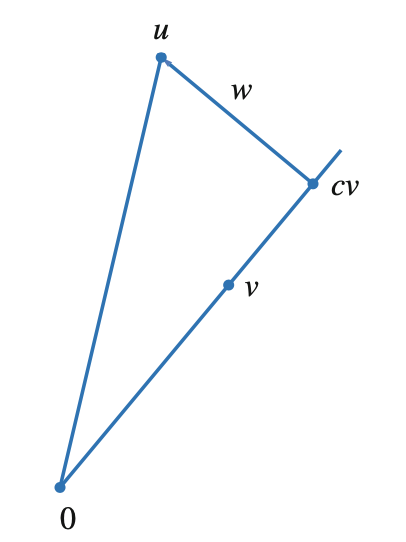
\includegraphics[width=0.25\textwidth]{axler6adecomp.png}
\end{figure}
In other words, we would like to \textit{decompose} $u$ into a vector $v$, plus some vector
orthogonal to $v$.

To do this, let $c\in \F$ denote a scalar. Then \[
  u = cv+(u-cv)
.\] Thus we need to choose $c$ so that $v$ is orthogonal to $u-cv$. In other words, we need \[
  0 =\left<u-cv,v \right> =\left<u,v \right> - c\left<v,v \right> =\left<u,v \right>-c\|v\|^2
.\] From this, we want \[
  c = \frac{\left<u,v \right>}{\|v\|^2}
.\] So, we can decompose $u$ into a scaled vector $v$, plus a vector $w=u-\frac{\left<u,v
\right>}{\|v\|^2}$ orthogonal to $v$: \[
  u = \frac{\left<u,v \right>}{\|v\|^2}v+\left(u-\frac{\left<u,v \right>}{\|v\|^2}v\right)
.\] In other words, we have proved the following result:
\begin{proposition}[Orthogonal Decomposition]{}
  Suppose $u,v\in V$ with $v\neq 0$. Set $c=\frac{\left<u,v \right>}{\left<v,v
  \right>}=\frac{\left<u,v \right>}{\|v\|^2}$, and $w=u-cv$. Then \[
    \left<w,v \right>=0 ~\text{and}~u=cv+w
  .\] 
\end{proposition}

If we only look at $cu$, this is essentially the value of the vector $v$ if \textbf{projected} onto
the vector $u$; that is, if we look at the value of $v$ only on $u$. This value has a special
name:
\begin{definition}[Projection]{}
  Let $u,v\in V$ with $v\neq 0$. The \textbf{projection of $v$ onto $u$}, denoted $\proj_{u}(v)$, is
  defined by \[
    \proj_{v}(u)=\frac{\left<u,v \right>}{\left<u,u \right>}u
  .\] We will see later that this has important implications for finding orthogonal bases.
\end{definition}

Orthogonal decomposition is quite useful, especially in the proof of the following important
equality:
\begin{proposition}[Cauchy-Schwarz Inequality]{}
  Suppose $u,v\in V$. Then \[
    \left| \left<u,v \right> \right|  \le \|u\|\|v\|=\left<u,u \right>\left<v,v \right>
  .\] Equality holds if and only if one vector is a scalar multiple of another.
\end{proposition}
\begin{proof}[Proof]
  If $v=0$, then both sides of the desired inequality equal $0$, so suppose $v\neq 0$. Consider \[
    u = \frac{\left<u,v \right>}{\left<v,v \right>}v+w
  \] given above, where $w$ is orthogonal to $v$. By the Pythagorean Theorem,
  \begin{align*}
    \|u\|^2&= \|\frac{\left<u,v \right>}{\left<v,v \right>}v\|^2+\|w\|^2 \\
           &= \frac{\left| \left<u,v \right> \right| ^2}{\left<v,v \right>}+\|w\|^2 \\
           &\ge \frac{\left| \left<u,v \right> \right| ^2}{\|v\|^2}
  .\end{align*} Hence \[
    \|u\|^2\|v\|^2 \ge \left| \left<u,v \right> \right| ^2
  ,\] and taking square roots then gives us the desired inequality.

  From the above proof, Cauchy-Schwarz is an equality if and only if this statement is an equality:
  \[
    \frac{\left| \left<u,v \right> \right| ^2}{\left<v,v \right>}+\left<w,w \right>\ge \frac{\left|
    \left<u,v \right> \right|^2 }{\left<v,v \right>}
  .\] Clearly, this is true only when $\left<w,w \right>=0$, or $w=0$. But $w=0$ if and only if $u$
  is a multiple of $v$ (geometrically, the orthogonal vector between $u$ and $v$ is $0$ only when
  one is a multiple of another). Thus equality holds if and only if one vector is a scalar multiple
  of another.
\end{proof}

The next result, called the \textbf{Triangle Inequality}, has the geometric interpretation that the
length of each side of a triangle is less than the sum of the lengths of the other two sides. This
also implies that the shortest path between two points is a line segment.

\begin{proposition}[Triangle Inequality]{}
  Suppose $u,v\in V$. Then \[
    \|u+v\|\le \|u\|+\|v\|
  .\] Again, equality holds if and only if one of $u,v$ is a non-negative multiple of another.
\end{proposition}
\begin{proof}[Proof]
  We have
  \begin{align*}
    \|u+v\|^2&= \left<u+v,u+v \right> \\
             &= \left<u,u \right>+\left<u,v \right>+\left<v,u \right>+\left<v,v \right> \\
             &= \left<u,u \right>+\left<v,v \right>+\left<u,v \right> +\overline{\left<u,v \right>}\\
             &\le  \|u\|^2+\|v\|^2+2\left| \left<u,v \right> \right|  \\
             &\le \|u\|^2+\|v\|^2+2\|u\|\|v\| \\
             &= (\|u\|+\|v\|)^2
  .\end{align*}
  The second last inequality comes from the Cauchy-Schwarz Inequality, and taking square roots thus
  gives the desired inequality: \[
    \|u+v\|\le \|u\|+\|v\|
  .\] 

  Equality holds if and only if $\left<u,v \right> =\|u\|\|v\|$; but this only holds if one is a
  scalar multiple of another. 
\end{proof}

This final result is called the parallelogram equality, because of its geometric interpretation: in
every parallelogram, the sum of the squares of the lengths of the diagonals equals the sum of the
squares of the lengths of the four sides.
\begin{figure}[htpb]
  \centering
  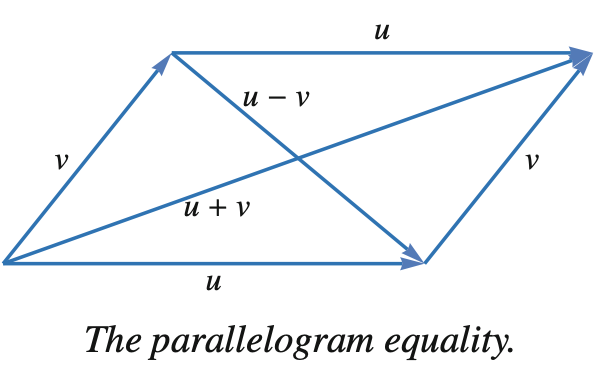
\includegraphics[width=0.25\textwidth]{axler6aparallelogram.png}
\end{figure}
\begin{proposition}[Parallelogram Equality]{}
  Suppose $u,v\in V$. Then \[
    \|u+v\|^2+\|u-v\|^2=2(\|u\|^2+\|v\|^2)
  .\] 
\end{proposition}
\begin{proof}[Proof]
  \begin{align*}
    \|u+v\|^2+\|u-v\|^2&= \left<u+v,u+v \right>+\left<u-v,u-v \right> \\
                       &= \|u\|^2+\|v\|^2+\left<u,v \right>+\left<v,u
                       \right>+\|u\|^2+\|v\|^2-\left<u,v \right>-\left<v,u \right>\\
                       &=2(\|u\|^2+\|v\|^2)
  ,\end{align*} as desired.
\end{proof}

\section{Orthonormal Bases}

\begin{definition}[Orthonormal]{}
  A list of vectors is called \textbf{orthonormal} if each vector in the list has norm $1$ and is
  orthogonal to all the other vectors in the list.

  In other words, a list $e_1,\ldots,e_m$ of vectors in $V$ is orthonormal if \[
    \left<e_j,e_k \right>=\left\{\begin{array}{rl} 1 & ~\text{if}~j=k,\\ 0 &~\text{if}~j\neq k
    \end{array}\right.\] 
\end{definition}

\begin{example}
  The standard basis in $\F^{n}$ is an orthonormal list. In addition, \[
    \left( \frac{1}{\sqrt{3}},\frac{1}{\sqrt{3}},\frac{1}{\sqrt{3}} \right), \left(- \frac{1}{\sqrt{2}},
    \frac{1}{\sqrt{2}}, 0\right), \left( \frac{1}{\sqrt{6}},\frac{1}{\sqrt{6}}, - \frac{2}{\sqrt{6}} \right) 
  \] is also an orthonormal list.
\end{example}

Why do we desire this result? It turns out that orthonormal lists are particularly easy to work
with.

\begin{proposition}[Norm of Orthonormal Linear Combination]{}
  If $e_1,\ldots,e_m$ is an orthonormal list of vectors in $V$, then \[
    \|a_1e_1+\ldots+a_me_m\|^2=\left| a_1 \right| ^2+\ldots+\left| a_m \right| ^2
  .\] 
\end{proposition}
\begin{proof}[Proof]
  Because each $e_j$ has norm $1$, this follows easily from repeated applications of the Pythagorean
  Theorem (which states that for orthogonal vectors $u,v\in V$, $\|u+v\|^2=\|u\|^2+\|v\|^2$; and the
  norm of a particular vector $\|a_ie_i\|^2=\left| a_i \right| ^2\|e_i\|^2=\left| a_i \right| ^2$).
\end{proof}

This result has the following important corollary.
\begin{corollary}[Orthonormal Lists are Linearly Independent]{}
  Every orthonormal list of vectors is linearly independent.
\end{corollary}
\begin{proof}[Proof]
  Suppose $e_1,\ldots,e_m$ is an orthonormal list of vectors in $V$ and $a_1,\ldots,a_m\in \F$ are
  such that \[
    a_1e_1+\ldots+a_me_m=0
  .\] Then $\left| a_1 \right|^2+\ldots+\left| a_m \right| ^2=0 $; but this is true only when every
  $a_i=0$. Thus $e_1,\ldots,e_m$ are linearly independent.
\end{proof}

Using this, we have the following definition.
\begin{definition}[Orthonormal Basis]{}
  An \textbf{orthonormal basis} of $V$ is an orthonormal list of vectors in $V$ that is also a basis
  of $V$.
\end{definition}
For instance, the standard basis of $\F^{n}$ is also an orthonormal basis.

Using linear independence of orthonormal lists, we get the following result:
\begin{proposition}{}
  Every orthonormal list of vectors in $V$ with length $\dim{V}$ is an orthonormal basis of $V$.
\end{proposition}

In general, given a basis $e_1,\ldots,e_m\in V$ and a vector $v\in V$, we know that there is some
choice of scalars $a_1,\ldots,a_m\in \F$ such that \[
  v=a_1e_1+\ldots+a_ne_n
.\] Computing the scalars $a_1,\ldots,a_m$ may be difficult for an arbitrary basis of $V$; however,
this is quite easy for an orthonormal basis: simply take \[
  a_j=\left<v,e_j \right>
!\] 

\begin{proposition}{}
  Suppose $e_1,\ldots,e_n$ is an orthonormal basis of $V$ and $v\in V$. Then \[
    v=\left<v,e_1 \right>e_1+\ldots+\left<v,e_n \right>e_n
  ,\] and \[
    \|v\|^2=\left| \left<v,e_1 \right> \right| ^2+\ldots+\left| \left<v,e_n \right> \right| ^2
  .\] 
\end{proposition}
\begin{proof}[Proof]
  Because $e_1,\ldots,e_m$ is a basis, there exist scalars $a_1,\ldots,a_n\in \F$ such that \[
    v=a_1e_1+\ldots+a_ne_n
  .\] Because $e_1,\ldots,e_n$ is orthonormal, taking the inner product with $e_j$ of both sides
  gives us \[
    \left<v,e_j \right> = a_1\left<e_1,e_j \right>+\ldots+a_n\left<e_n,e_j \right>
  .\] But $\left<e_i,e_j \right>=0$, unless $i=j$, in which case it equals $1$; thus \[
    \left<v,e_j \right>=a_j
  .\]

  The second equation follows immediately from above, and the previous proposition.
\end{proof}

Now that we see the usefulness of orthonormal bases, how do we find them? For example, does
$\mc{P}_m(\R)$ have an orthonormal basis? The following result will provide a procedural method to
generating orthonormal bases from linearly independent bases.

\begin{theorem}[Gram-Schmidt Procedure]{}
  Suppose $v_1,\ldots,v_m$ is a linearly independent list of vectors in $V$. Let
  $e_1=\frac{v_1}{\|v_1\|}$. For $j=2,\ldots,m$, define $e_j$ inductively by \[
    e_j=\frac{v_j-\left<v_j,e_1 \right>e_1-\ldots-\left<v_j,e_{j-1}
    \right>e_{j-1}}{\|v_j-\left<v_j,e_1 \right>e_1-\ldots-\left<v_j,e_{j-1} \right>e_{j-1}\|}
  .\] Then $e_1,\ldots,e_m$ is an orthonormal list of vectors in $V$ such that \[
  \Span{(v_1,\ldots,v_j)}=\Span{(e_1,\ldots,e_j)}
  \] for $j=1,\ldots,m$.
\end{theorem}
\begin{proof}[Proof]
  We show by induction on $j$ that the desired conclusion holds. For $j=1$,
  $\Span{(v_1)}=\Span{(e_1)}$, since $ v_1$ is a positive multiple of $e_1$.

  Suppose $1<j<m$ and \[
    \Span{(v_1,\ldots,v_{j-1})}=\Span{(e_1,\ldots,e_{j-1})}
  \] holds. Note that $v_j\not\in \Span{(v_1,\ldots,v_{j-1})}$, since $v_1,\ldots,v_m$ is linearly
  independent; thus $v_j\not\in \Span{(e_1,\ldots,e_{j-1})}$ either. Hence in the definition above,
  we are not dividing by zero, since $v_j$ not in span means it is impossible for
  $v_j-\sum_{i=1}^{j-1} a_ie_i$ to be zero either. Dividing a vector by its norm produces a new
  vector with norm $1$; thus $\|e_j\|=1$.

  Let $1\le k<j$. Then
  \begin{align*}
    \left<e_j,e_k \right> &= \left<\frac{v_j-\left<v_j,e_1 \right>e_1-\ldots-\left<v_j,e_{j-1}
    \right>e_{j-1}}{\|v_j-\left<v_j,e_1 \right>e_1-\ldots-\left<v_j,e_{j-1} \right>e_{j-1}\|},e_k \right> \\
    &= \frac{\left<v_j,e_k \right>-\left<v_j,e_k \right>}{\|v_j-\left<v_j,e_1 \right>e_1-\ldots-\left<v_j,e_{j-1} \right>e_{j-1}\|} \\
    &=0
  ,\end{align*}
  where the second last step follows because $\left<e_j,e_k \right>=0$ for all $j\neq k$. Thus $e_j$
  is orthonormal to all previous vectors, and so $e_1,\ldots,e_j$ is an orthonormal list.

  From the above definition of $e_j$, we see that $v_j\in \Span{(e_1,\ldots,e_j)}$. Since we've
  assumed that $\Span{(e_1,\ldots,e_{j-1})}=\Span{(v_1,\ldots,v_{j-1})}$, we thus get \[
    \Span{(v_1,\ldots,v_j)}\subset\Span{(e_1,\ldots,e_j)}
  .\] Both lists above are linearly independent ($v$'s given, $e$'s by orthonormality). Therefore
  both of these subspaces have dimension $j$, and hence they are equal.
\end{proof}

This definition of $e_j$ seems extremely complicated, at first glance. However, closer inspection
reveals somewhat of an intuitive process:
\begin{itemize}
  \item First, we wish to convert a list of linearly independent vectors into a list of orthonormal
    vectors. Let's first forget about orthonormality, and look solely at orthogonality.
  \item We can start with any one vector; this will be the ``base'' vector, $v_1=u_1$. In order to find
    the next \textit{orthogonal} vector, we must find a vector orthogonal to $u_1$:
    \begin{itemize}
      \item Recall that a vector $v_2\in V$ can be decomposed into $u_1$, plus a vector orthogonal
        to it. To do this, we convert $v_2$ into $\frac{\left<u_1,v_2 \right>}{\left<u_1,u_1
        \right>}u_1+w$, where $w$ is the vector orthogonal to $u_1$. \textbf{This is the vector
      we're interested in!}
    \end{itemize}
    Thus, using orthogonal decomposition, we simply want the vector orthogonal to the base vector
    $u_1$, and so we get \[
      u_2=w=v_2-\frac{\left<u_1,v_2 \right>}{\left<u_1,u_1 \right>}u_1=v_2-\proj_{u_1}(v_2)
    .\] 
  \item Now, we wish to repeat this process with the rest of the vectors $v_i$. Like before, we wish
    to find a vector orthogonal to every other vector. We can repeat the processes above
    iteratively, by finding a vector (say $v_i'$) orthogonal to one vector (say $u_1$), then using
    that to find another vector (say $v_i''$) orthogonal to both $u_1$ and another vector (say
    $u_2$), and so on until we reach a vector $u_i$ orthogonal to all previous $u_{1\le j<i}$. This
    gives us the desired (if complex) formula,
    \begin{align*}
      u_j&=v_j-\proj_{u_1}(v_j)-\proj_{u_2}(v_j)-\ldots-\proj_{u_{j-1}}(v_j)\\
         &=v_j-\frac{\left<u_1,v_j \right>}{\left<u_1,u_1 \right>}u_1-\ldots-\frac{\left<u_{j-1},v_j
         \right>}{\left<u_{j-1},u_{j-1} \right>}u_{j-1}
    .\end{align*}
  \item This process gives us a list of \textit{orthogonal} vectors; but if we desire an orthonormal
    list, we need the extra step of dividing by the norm of the result. Luckily, if each $u_j$ is
    orthogonal, then every $\left<u_j,u_j \right>=1$, so we can focus only on the numerator. That's
    how we arrive at the final equation, \[
      e_j=\frac{v_j-\left<v_j,e_1 \right>e_1-\ldots-\left<v_j,e_{j-1}
      \right>e_{j-1}}{\|v_j-\left<v_j,e_1 \right>e_1-\ldots-\left<v_j,e_{j-1} \right>e_{j-1}\|}
    .\] 
\end{itemize}


Let's look at an example of the Gram-Schmidt process in action.
\begin{example}
  Find the orthonormal basis of $\mc{P}_2(\R)$, where the inner product is given by \[
    \left<p,q \right>=\int_{-1}^{1}p(x)q(x)dx
  .\] 
\end{example}
\begin{solution}
  We apply the Gram-Schmidt procedure to the basis $1,x,x^2$.

  We have \[
    e_1=\frac{1}{\|1\|}=\frac{1}{\sqrt{\int_{-1}^11^2dx}}=\frac{1}{\sqrt{2}}
  .\] Now, the numerator for $e_2$ is \[
  x-\left<x,e_1 \right>e_1=x-\left( \int_{-1}^1x\frac{1}{\sqrt{2}}dx \right)\frac{1}{\sqrt{2}}=x
  ;\] moreover, \[
    \|x\|^2=\int_{-1}^1x^2dx=\frac{2}{3}
  .\] Thus $\|x\|=\sqrt{\frac{2}{3}}$, and so
  $e_2=\frac{x}{\sqrt{\frac{2}{3}}}=x\sqrt{\frac{3}{2}}$.

  Finally, the numerator for $e_3$ is
  \begin{align*}
    x^2&-\left<x^2,e_1 \right>e_1-\left<x^2,e_2 \right>e_2\\
       &= x^2-\left( \int_{-1}^1x^2\sqrt{\frac{1}{2}}dx\right)-\left(
       \int_{-1}^1x^2\sqrt{\frac{3}{2}}dx \right) x\sqrt{\frac{3}{2}}\\
       &= x^2-\frac{1}{3}
  .\end{align*}
  Moreover, \[
    \|x^2-\frac{1}{3}\|^2=\int_{-1}^1(x^4-\frac{2}{3}x^2+\frac{1}{9})dx=\frac{8}{45}
  .\] Thus $\|x^2-\frac{1}{3}\|=\sqrt{\frac{8}{45}}$, and so
  $e_3=\sqrt{\frac{45}{8}}(x^2-\frac{1}{3})$.

  Thus \[
    \frac{1}{\sqrt{2}},\ x\sqrt{\frac{3}{2}},\sqrt{\frac{45}{8}}(x^2-\frac{1}{3})
  \] is an orthonormal basis of $\mc{P}_2(\R)$.
\end{solution}

But do these orthonormal bases always exist? It turns out that yes, they do.
\begin{proposition}[Existence of Orthonormal Basis]{}
  Every finite-dimensional inner product space has an orthonormal basis.
\end{proposition}
\begin{proof}[Proof]
  Suppose $V$ is finite-dimensional. Choose a basis of $V$. Apply the Gram-Schmidt procedure to it,
  producing an orthonormal list with length $\dim{V}$. From before, we see that any orthonormal list
  of the right length ($\dim{V}$) is an orthonormal basis of $V$.
\end{proof}

Not only does an orthonormal basis always exist, we can also extend an orthonormal list of vectors
to an orthonormal basis, using the Gram-Schmidt procedure.
\begin{corollary}[Orthonormal List Extends to Orthonormal Basis]{}
  Suppose $V$ is finite-dimensional. Then every orthonormal list of vectors in $V$ can be extended
  to an orthonormal basis of $V$.
\end{corollary}
\begin{proof}[Proof]
  Suppose $e_1,\ldots,e_m$ is an orthonormal list of vectors in $V$. Then $e_1,\ldots,e_m$ is
  linearly independent, and thus this list can be extended to a basis \[
    e_1,\ldots,e_m, v_1,\ldots,v_n
  \] of $V$. Now, using the Gram-Schmidt procedure we can produce an orthonormal list \[
    e_1,\ldots,e_m,f_1,\ldots,f_n
  ;\] the first $m$ vectors remain unchanged since they're already orthonormal. Then the list is an
  orthonormal basis.
\end{proof}

Now, let's explore some connections between orthonormal lists and upper-triangular matrices. We've
shown before that every operator $T\in \mc{L}(V)$ has a basis that produces an upper-triangular
matrix for $\mc{M}(T)$. Now, with inner product spaces, we're interested in whether there's an
\textbf{orthonormal} basis that produces an upper-triangular matrix.

With Gram-Schmidt, our wishes are fulfilled; as long as a basis admits an upper-triangular matrix,
then we have what we need (this is always true for complex vector spaces, but only sometimes true
for real vector spaces).
\begin{proposition}[Upper-Triangular w.r.t. Orthonormal Basis]{}
  Suppose $T\in \mc{L}(V)$. If $T$ has an upper-triangular matrix with respect to some basis of $V$,
  then $T$ has an upper-triangular matrix with respect to some orthonormal basis of $V$.
\end{proposition}
\begin{proof}[Proof]
  Suppose $T$ has an upper-triangular matrix with respect to some basis $v_1,\ldots,v_n\in V$. Thus
  $\Span{(v_1,\ldots,v_j)}$ is invariant under $T$ for each $1\le j\le n$.

  Applying Gram-Schmidt to $v_1,\ldots,v_n$, we get an orthonormal basis $e_1,\ldots,e_n\in V$.
  Since \[
    \Span{(e_1,\ldots,e_n)}=\Span{(v_1,\ldots,v_n)}
  ,\] we conclude that $\Span{(e_1,\ldots,e_n)}$ is invariant under $T$. Thus $T$ has an
  upper-triangular matrix with respect to the orthonormal basis $e_1,\ldots,e_n$.
\end{proof}

This next result is an important application of the above result:
\begin{theorem}[Schur's Theorem]{}
  Suppose $V$ is a finite-dimensional complex vector space and $T\in \mc{L}(V)$. Then $T$ has an
  upper-triangular matrix with respect to some orthonormal basis of $V$.
\end{theorem}
\begin{proof}[Proof]
  Recall that $T$ has an upper-triangular matrix with respect to some basis of $V$ (since every
  operator in a complex vector space admits an upper-triangular matrix). Then, from above, $T$ has
  an upper-triangular orthonormal basis.
\end{proof}

\subsection{Linear Functionals on Inner Product Spaces}

Since linear maps into the scalar field $\F$ play an important role, we give them a special name.
\begin{definition}[Linear Functional]{}
  A \textbf{linear functional} on $V$ is a linear map from $V$ to $\F$. In other words, a linear
  functional is an element of $\mc{L}(V,\F)$.
\end{definition}
\begin{example}
  The function $\varphi:\F^3\to \F$ defined by \[
    \varphi(z_1,z_2,z_3)=2z_1-5z_2+z_3
  \] is a linear functional on $\F^3$. We could write this linear functional in the form \[
  \varphi(z)=\left<z,u \right>
\] for every $z\in \F^3$, where $u=(2,-5,1)$ (recall that unless explicitly stated otherwise, the
default inner product for $\F^n$ is the Euclidean inner product; and every vector space is naturally
an inner product space).
\end{example}

\begin{example}
  The function $\varphi:\mc{P}_2(\R)\to \R$ defined by \[
    \varphi(p)=\int_{-1}^1p(t)\left( \cos{\pi(t)} \right) dt
  \] is a linear functional on $\mc{P}_2(\R)$ (here the inner product is multiplication followed by
  integration on $[-1,1]$). It's not obvious that there exists a $u\in \mc{P}_2(\R)$ that satisfies
  \[
    \varphi(p)=\left<p,u \right>
  \] for every $p\in \mc{P}_2(\R)$, since we cannot take $u(t)=\cos{(\pi t)}\not\in \mc{P}_2(\R)$.
\end{example}

If $u\in V$, then the map that sends $v$ to $\left<v,u \right>$ is a linear functional on $V$. The
next result shows that \textbf{every linear functional on $V$ is of this form}! This result is
indeed powerful; the above example demonstrates that there's not always an obvious candidate for
$u$.

\begin{theorem}[Riesz Representation Theorem]{}
  Suppose $V$ is finite-dimensional and $\varphi$ is a linear functional on $V$. Then there is a
  unique vector $u\in V$ such that \[
    \varphi(v)=\left<v,u \right>
  \] for every $v\in V$ (here, the inner product is the underlying inner product of the inner
  product space $V$).
\end{theorem}
\begin{proof}[Proof]
  First, we show existence. Let $e_1,\ldots,e_n$ be an orthonormal basis for $V$. Then
  \begin{align*}
    \varphi(v)&= \varphi(\left<v,e_1 \right>e_1+\ldots+\left<v,e_n \right>e_n) \\
              &= \left<v,e_1 \right>\varphi(e_1)+\ldots+\left<v,e_n \right>\varphi(e_n) \\
              &= \left<v,\overline{\varphi(e_1)}e_1 \right>+\ldots+\left<v,\overline{\varphi(e_n)}
              e_n\right> \\
              &= \left<v,\overline{\varphi(e_1)}e_1+\ldots+\overline{\varphi(e_n)}e_n \right>
  \end{align*}
  for every $v\in V$ (recall that any $v$ can be represented as $\left<v,e_1
  \right>e_1+\ldots+\left<v,e_n \right>e_n$ if $e_1,\ldots,e_n$ is an orthonormal basis; and inner
  products are conjugate-linear with respect to their second terms). Thus setting \[
    u = \overline{\varphi(e_1)}e_1+\ldots+\overline{\varphi(e_n)}e_n
  ,\] we have $\varphi(v)=\left<v,u \right>$, as desired.

  Now, we show uniqueness. Suppose $u_1,u_2\in V$ such that \[
    \varphi(v)=\left<v,u_1 \right>=\left<v,u_2 \right>
  \] for every $v\in V$. Then \[
    0=\left<v,u_1 \right>-\left<v,u_2 \right> = \left<v,u_1-u_2 \right>
  \] for every $v\in V$. Taking $v=u_1-u_2$, properties of inner product spaces tells us that
  $v=u_1-u_2=0$; thus $u1=u_2$, and we get uniqueness.
\end{proof}

Not only does this prove the existence and uniqueness of $u\in V$ that satisfies \[
  \varphi(v)=\left<v,u \right>
\] for all $v\in V$, this also provides a formula for finding $u$: \[
    u = \overline{\varphi(e_1)}e_1+\ldots+\overline{\varphi(e_n)}e_n
.\] This seems to imply that $u$ is dependent on the choice of orthonormal basis $e_1,\ldots,e_n$,
as well as $\varphi$; but the Reisz Representation Theorem tells us that $u$ is uniquely determined
by $\varphi$; thus $u$ is invariant of chosen orthonormal basis $e_1,\ldots,e_n$ of $V$.

\begin{example}
  Find $u\in \mc{P}_2(\R)$ such that \[
    \int_{-1}^1p(t)(\cos{(\pi t)})dt=\int_{-1}^1p(t)u(t)dt
  \] for all $p\in \mc{P}_2(\R)$.
\end{example}
\begin{solution}
  Let $\varphi(p)=\int_{-1}^1p(t)(\cos{\pi t})dt$. Using the formula above and the orthonormal basis
  from the previous example, we have
  \begin{align*}
    u(x)&= \left( \int_{-1}^1\sqrt{\frac{1}{2}}(\cos{(\pi t)})dt \right)\sqrt{\frac{1}{2}} +\left(
    \int_{-1}^1\sqrt{\frac{3}{2}}t(\cos{(\pi t)})dt \right) \sqrt{3/2}x \\
        &+\left( \int_{-1}^1\sqrt{\frac{45}{8}}(t^2-\frac{1}{3})(\cos{(\pi t)})dt \right)
        \sqrt{\frac{45}{8}}(x^2-\frac{1}{3})
  .\end{align*}
  A little bit of calculus (:tf:) shows that \[
    u(x)=-\frac{45}{2\pi^2}(x^2-\frac{1}{3})
  .\] 
\end{solution}


\section{Orthogonal Complements and Minimization Problems}

\subsection{Orthogonal Complements}
\begin{definition}[Orthogonal Complement]{}
  If $U$ is a subset of $V$, then the \textbf{orthogonal complement} of $U$, denoted $U^{\bot}$, is
  the set of all vectors in $V$ that are orthogonal to every vector in $U$: \[
    U^{\bot}=\{v\in V\mid \left<v,u \right> =0~\text{for every}~u\in U\} 
  .\]
\end{definition}
For example, if $U$ is a line in $\R^3$, then $U^{\bot}$ is the plane containing the origin that is
perpendicular to $U$. If $U$ is instead a plane in $\R^3$, then $U^{\bot}$ is the line containing
the origin that is perpendicular to $U$.
\begin{proposition}[Properties of Orthogonal Complements]{}
  \begin{enumerate}
    \item If $U$ is a subset of $V$, then $U^{\bot}$ is a subspace of $V$.
    \item $\{ 0 \}^{\bot}=V$.
    \item $V^{\bot}=\{ 0 \}$.
    \item If $U$ is a subset of $V$, then $U\cap U^{\bot}\subseteq \{ 0 \}$.
    \item If $U$ and $W$ are subsets of $V$ and $U\subseteq W$, then $W^{\bot}\subseteq U^{\bot}$.
  \end{enumerate}
\end{proposition}
\begin{proof}[Proof]
  \begin{enumerate}
    \item Suppose $U$ is a subset of $V$. Then $\left<0,u \right> =0$ for every $u\in U$; thus $0\in
        U^{\bot}$.
      Suppose $v,w\in U^{\bot}$. If $u\in U$, then \[
        \left<v+w,u \right> =\left<v,u \right> +\left<w,u \right> =0+0=0
      .\] Thus $v+w\in U^{\bot}$.
      Finally, suppose $\lambda\in \F,\ v\in U^{\bot}$. If $u\in U$, then \[
        \left<\lambda v,u \right> =\lambda\left<v,u \right> =\lambda\cdot 0=0
      .\] Thus $\lambda v\in U^{\bot}$, and so $U^{\bot}$ is a subspace of $V$.

    \item Clearly, any $v\in V$ satisfies $\left<v,0 \right> =0$. Thus every $v\in V^{\bot}$, so
      $V^{\bot}=V$.
    \item Suppose $v\in V^{\bot}$. Then $\left<v,v \right> =0$, which forces $v=0$. Thus
      $V^{\bot}=\{ 0 \}$.
    \item Suppose $U$ is a subset of $V$ and $v\in U\cap U^{\bot}$. Then $\left<v,v \right> =0$,
      which forces $v=0$. Thus $U\cap U^{\bot}\subseteq \{ 0 \}$.
    \item Suppose $U,W$ are subsets of $V$ and $U\subseteq W$. Suppose $v\in W^{\bot}$. Since $u\in
      U\subseteq W$, $\left<v,u \right> =0$ for every $u\in U$. Thus $W^{\bot}\subseteq U^{\bot}$.
  \end{enumerate}
\end{proof}

With direct sums, we can start to see why it is referred to as the orthogonal complement. Suppose
$U$ and $W$ are subspaces of $V$ such that $U\oplus W=V$ (in other words, every vector $v\in V$ can
be written in exactly one way as a vector in $U$ plus a vector in $V$). It turns out that every
vector space can be decomposed into a subspace and its orthogonal complement.

\begin{theorem}[Direct Sum of Subspace and Orthogonal Complement]{}
  Suppose $U$ is a finite-dimensional subspace of $V$. Then \[
    V=U\oplus U^{\bot}
  .\]
\end{theorem}
\begin{proof}[Proof]
  First, we will show that $V=U+U^{\bot}$. Suppose $v\in V$, and suppose $e_1,\ldots,e_m\in U$ is an
  orthonormal basis of $U$. Clearly, \[
    v=\underbrace{\left<v,e_1 \right> e_1+\ldots+\left<v,e_m \right> e_m}_u
    +\underbrace{v-\left<v,e_1 \right>e_1-\ldots-\left< v,e_m\right>e_m}_w
  .\] Let $u$ and $w$ be vectors as defined above. Clearly, $u\in U$. Since $e_1,\ldots,e_m$ is an
  orthonormal list, for each $j=1,\ldots,m$ we have \[
    \left<w,e_j \right> =\left<v,e_j \right> -\left<v,e_j \right> =0
  .\] This is because taking the inner product of $w$ with respect to $e_j$ gives us $\left<v,e_j
  \right> -\left<v,e_j \right> \left<e_j,e_j \right> =\left<v,e_j \right> -\left<v,e_j \right> $,
  since $\left<e_j,e_j \right> =1$ and $\left<e_j,e_k \right> =0$ for every $j\neq k$.

  Thus $w$ is orthogonal to every vector in $\Span{(e_1,\ldots,e_m)}$. In other words, $w\in
  U^{\bot}$. Thus we have written any vector $v\in V$ as $v=u+w$, where $u\in U$ and $w\in
  U^{\bot}$.

  From the properties shown above, we know $U\cap U^{\bot}=\{ 0 \}$. By Proposition 1.45 and above,
  we see that $V=U\oplus U^{\bot}$.
\end{proof}

Now, computing $\dim{U^{\bot}}$ is trivial; simply take \[
  \dim{U^{\bot}}=\dim{V}-\dim{U}
.\] Another important consequence of the theorem is the following:
\begin{proposition}{}
  Suppose $U$ is a vinite-dimensional subspace of $V$. Then \[
    U=\left( U^{\bot} \right) ^\bot
  .\] 
\end{proposition}
\begin{proof}[Proof]
  First, we show that \[
    U\subseteq \left( U^{\bot} \right) ^\bot
  .\] Suppose $u\in U$. Then $\left<u,v \right> =0$ for every $v\in U^{\bot}$ (by definition). Since
  $u$ is thus orthogonal to every vector in $U^{\bot}$, we have $u\in \left( U^{\bot} \right)
  ^\bot$.

  To show $\left( U^{\bot} \right) ^\bot\subseteq U$, suppose $v\in \left( U^{\bot} \right) ^\bot$.
  We can write $v=u+w$ (since the complement of a subset, here $U^{\bot}$, is a subspace of $V$),
  where $u\in U$ and $w\in U^{\bot}$. Then \[
    w=v-u\in U^{\bot}
  .\] Since $v\in \left( U^{\bot} \right) ^bot$ and $u\in \left( U^{\bot} \right)^\bot$ (from above,
  since $U\subseteq \left( U^{\bot} \right) ^\bot$), we have $v-u\in \left( U^{\bot} \right) ^\bot$.
  But this means $v-u\in U^{\bot}\cap \left( U^{\bot} \right) ^\bot$, which implies that $v-u$ is
  orthogonal to itself; in other words, $\left<v-u,v-u \right> =0$, so $v-u=0$, and so $v=u\in U$,
  so $v\in U$ as well. Thus every vector in $\left( U^{\bot} \right) ^\bot$ is in $U$ as well, so
  $\left( U^{\bot} \right) ^\bot\subseteq U$, completing the proof.
\end{proof}

We now define an operator $\mc{P}_U$ for every finite-dimensional subspace $U$ of $V$.

\begin{definition}[Orthogonal Projection]{}
  Suppose $U$ is a finite-dimensional subspace of $V$. The \textbf{orthogonal projection of $V$ onto
  $U$} is the operator $\mc{P}_U\in \mc{L}(V)$, defined as follows: \begin{center}
    For $v\in V$, write $v=u+w$ where $u\in U$ and $w\in U^{\bot}$. Then $\mc{P}_U(v)=u$.
  \end{center}
\end{definition}

Since given a subpsace, every vector space uniquely decomposes into that subspace and its orthogonal
complement, $\mc{P}_U$ is well-defined.

\begin{example}
  Suppose $x\in V$ with $x\neq 0$ and $U=\Span{(x)}$. Show that \[
    \mc{P}_U(v)=\frac{\left<v,x \right> }{\|x\|^2}x
  \] for every $v\in V$.
\end{example}
\begin{solution}
  Suppose $v\in V$. Then \[
    v=\frac{\left<v,v \right> }{\|x\|^2}x+\left( v-\frac{\left<v,x \right> }{\|x\|^2}x \right) 
  ,\] where the first term on the right is in $\Span{(x)}$ (and thus in $U$) and the second term on
  the right is orthogonal to $x$ (see the proof of the direct sum theorem above for why), and thus
  in $U^{\bot}$. Thus $\mc{P}_U(v)$ equals the first term on the right, as desired.
\end{solution}

\begin{proposition}[Properties of Orthogonal Projections]{}
  Suppose $U$ is a finite-dimensional subspace of $V$ and $v\in V$. Then
  \begin{enumerate}
    \item $\mc{P}_U\subseteq \mc{L}(V)$;
    \item $\mc{P}_Uu=u$ for every $u\in U$;
    \item $\mc{P}_Uw=0$ for every $w\in U^{\bot}$;
    \item $\range{\mc{P}_U}=U$;
    \item $\Null{\mc{P}_U}=U^{\bot}$;
    \item $v-\mc{P}_Uv\in U^{\bot}$;
    \item $\mc{P}_U^2=\mc{P}_U$;
    \item $\|\mc{P}_Uv\|\le \|v\|$;
    \item For every orthonormal basis $e_1,\ldots,e_m\in U$, \[
      \mc{P}_Uv=\left<v,e_1 \right>e_1+\ldots+\left<v,e_m \right> e_m 
    .\] 
  \end{enumerate}
\end{proposition}
\begin{proof}[Proof]
  \begin{enumerate}
    To show that $\mc{P}_U$ is a linear map on $V$, suppose $v_1,v_2\in V$. Write them as \[
        v_1=u_1+w_1,\ v_2=u_2+w_2
      ,\] where $u_1,u_2\in U$ and $w_1,w_2\in U^{\bot}$. Thus $\mc{P}_Uv_1=u_1$ and $\mc{P}_Uv_2=u_2$.
      Since $v_1+v_2=(u_1+u_2)+(w_1+w_2)$, clearly \[
        \mc{P}_U(v_1+v_2)=u_1+u_2=\mc{P}_Uv_1+\mc{P}_Uv_2
      .\] Similarly with $\lambda\in \F$, $\lambda v_1=\lambda u_1+\lambda w_1$, so \[
      \mc{P}_U(\lambda v_1)=\lambda u_1=\lambda\mc{P}_Uv_1
      .\] Thus $\mc{P}_U\in \mc{L}(V)$ is a valid linear map.

      All but the last two follow trivially.

      For the second last one, let $v=u+w$ with $u\in U,\ w\in U^{\bot}$. Then \[
        \|\mc{P}_Uv\|^2=\|u\|^2\le \|u\|^2+\|w\|^2=\|v\|^2
      ,\] where the last equality comes from the Pythagorean Theorem.

      The last property follows from the proof of the direct sum decomposition.
    
  \end{enumerate}
\end{proof}

\subsection{Minimization Problems}

This problem often arises: given a subspace $U$ of $V$ and a point $v\in V$, find a point $u\in U$
such that $\|v-u\|$ is as small as possible. It turns out that this minimization problem is actually
solved by taking $u=\mc{P}_Uv$.

\begin{proposition}[Minimizing Distance to Subspace]{}
  Suppose $U$ is a finite-dimensional subspace of $V$, $v\in V$, and $u\in U$. Then \[
    \|v-\mc{P}_Uv\|\le \|v-u\|
  .\] In other words, the distance between $v$ and $\mc{P}_Uv$ is smaller than the distance between
  $v$ and any vector $u$ in $U$. Equality only holds if $u=\mc{P}_Uv$.
\end{proposition}
\begin{proof}[Proof]
  We have
  \begin{align*}
    \|v-\mc{P}_Uv\|^2&\le \|v-\mc{P}_Uv\|^2+\|\mc{P}_Uv-u\|^2\\
                     &=\|(v-\mc{P}_Uv)+(\mc{P}_Uv-u)\|^2\\
                     &=\|v-u\|^2
  .\end{align*}
  The first inequality holds because $\|\mc{P}_Uv-u\|^2\ge 0$, and the secone equality holds due to
  the Pythagorean Theorem (since $v-\mc{P}_Uv\in U^{\bot}$, and $\mc{P}_Uv-u\in U$). Taking square
  roots gives the desired inequality.

  Inequality becomes equality if and only if the above inequality is an equality, which happens if
  and only if $\mc{P}_Uv-u=0$, or $\mc{P}_Uv=u$.
\end{proof}






 



























\end{document}
